\section{Model-wide zero-product accounting}
\label{sec:measurement}

Let a scalar product be a multiplication between two scalar operands within a
declared matrix product.  For operation $o$, let $N_o$ be the number of such
products in the evaluated workload and $Z_o$ the number for which at least one
\emph{measured} operand is exactly zero.  We count six operations in each
Pythia block: fused QKV projection, causal QK scores, causal probability--value
(PV) products, attention output projection, and the MLP up and down
projections.  Future positions are excluded from both QK and PV denominators.
The language-model head is declared dense and contributes $N_{\rm head}$ only
to the denominator:
\begin{equation}
 \Rmodel =
 \frac{\sum_{\ell=1}^{L}\sum_o Z_{\ell,o}}
 {\sum_{\ell=1}^{L}\sum_o N_{\ell,o}+N_{\rm head}}.
 \label{eq:rmodel}
\end{equation}
Counts are accumulated as integers over all sequences and layers before the
division.  We use ``model-wide'' to mean this declared graph and workload, not
all possible implementations of a language model.

For sequence length $T$, hidden width $d$, and MLP width $d_f$, the dense
per-block denominator is
\begin{equation}
 N_{\rm block}=T(4d^2+2dd_f)+dT(T+1),
 \label{eq:denominator}
\end{equation}
where the final term combines the two valid-causal attention products.  The
model denominator is $L N_{\rm block}+TdV$ for vocabulary size $V$.  The metric
is evaluated under eager attention so that the operands immediately before
each product are observable.

This definition resolves three ambiguities in local sparsity.  First, it
weights zeros by exact operation footprints rather than by tensor size alone.
Second, it counts reuse: one key or value coordinate can zero products at many
valid query positions.  Third, it places the observation after any intervening
transformation.  In particular, query and key are measured after partial RoPE;
a zero before RoPE is not credited merely because it was once zero.  Conversely,
$\Rmodel$ does \emph{not} estimate wall-clock acceleration.  A dense kernel may
execute every counted product, and sparse kernels face indexing, load balance,
and shape-dependent overheads.

For descriptive context we also compute a topology-conditioned analytic reach
$\Rmax$: the share of the same denominator belonging to operations that would
become all-zero if the topology's selected sites were all zero.  It is neither
an observed zero rate nor a universal upper bound on measured $\Rmodel$, since
the latter includes natural zeros at unselected operands.  We therefore do not
use its normalization as a primary result.

\begin{figure*}[t]
  \centering
  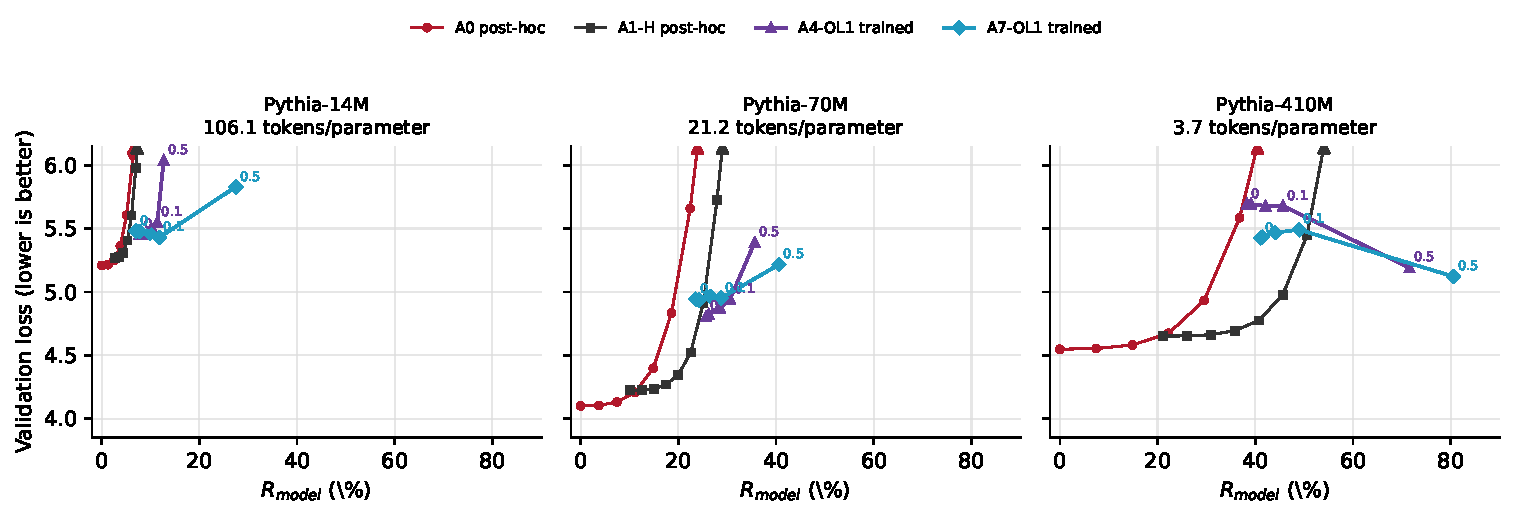
\includegraphics[width=\textwidth]{figures/01-absolute-frontiers-by-scale.pdf}
  \caption{Validation loss versus measured model-wide zero-product opportunity.
  Lines connect gate thresholds (trained) or clipping targets (post-hoc); they
  are not fitted scaling curves.  Upward triangles at the plot boundary mark
  post-hoc points whose losses exceed the displayed range.  All points use one
  seed and complete validation.}
  \label{fig:absolute}
\end{figure*}

